\documentclass{standalone}
\usepackage{tikz}
\usetikzlibrary{shapes, arrows.meta, positioning}

\begin{document}

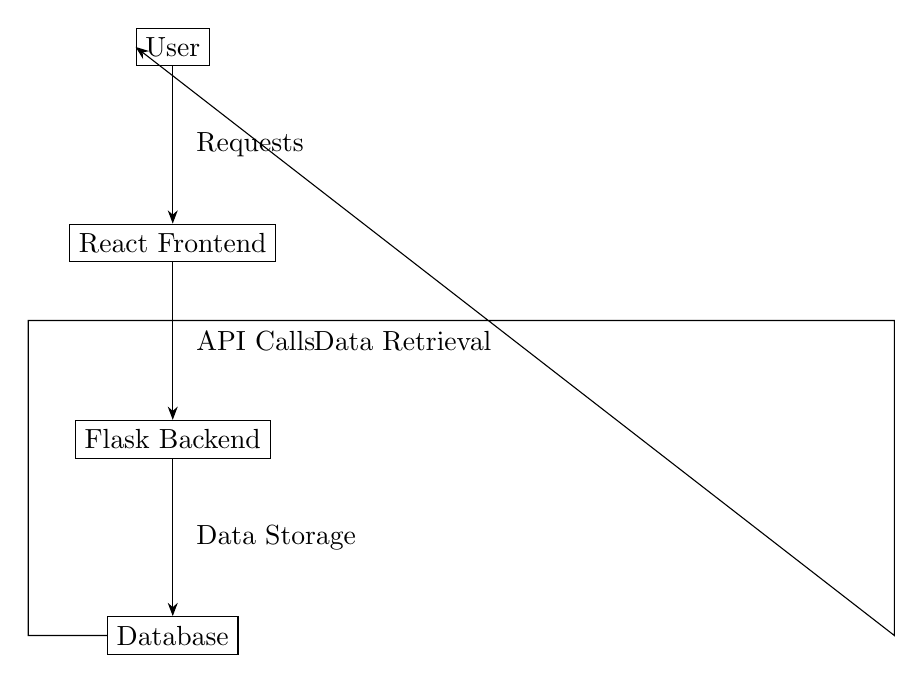
\begin{tikzpicture}[>=Stealth, node distance=2cm]

% Nodes
\node (user) [draw, rectangle, align=center] {User};
\node (frontend) [draw, rectangle, below=of user, align=center] {React Frontend};
\node (backend) [draw, rectangle, below=of frontend, align=center] {Flask Backend};
\node (database) [draw, rectangle, below=of backend, align=center] {Database};

% Arrows
\draw[->] (user) -- (frontend) node[midway, right, xshift=5pt] {Requests};
\draw[->] (frontend) -- (backend) node[midway, right, xshift=5pt] {API Calls};
\draw[->] (backend) -- (database) node[midway, right, xshift=5pt] {Data Storage};
\draw[->] (database.west) -- ++(-1,0) -- ++(0,4) -- ++(11,0) -- ++(0,-4) -- (user.west) node[midway, left, xshift=-5pt] {Data Retrieval};

\end{tikzpicture}

\end{document}
